%%%%%%%% ICML 2021 EXAMPLE LATEX SUBMISSION FILE %%%%%%%%%%%%%%%%%

\documentclass{article}

% Recommended, but optional, packages for figures and better typesetting:
\usepackage{microtype}
\usepackage{graphicx}
\usepackage{subfigure}
\usepackage{booktabs} % for professional tables

% hyperref makes hyperlinks in the resulting PDF.
% If your build breaks (sometimes temporarily if a hyperlink spans a page)
% please comment out the following usepackage line and replace
% \usepackage{icml2021} with \usepackage[nohyperref]{icml2021} above.
\usepackage{hyperref}

% Attempt to make hyperref and algorithmic work together better:
\newcommand{\theHalgorithm}{\arabic{algorithm}}

% Use the following line for the initial blind version submitted for review:
%\usepackage{icml2021}

% If accepted, instead use the following line for the camera-ready submission:
\usepackage[accepted]{icml2021}

% The \icmltitle you define below is probably too long as a header.
% Therefore, a short form for the running title is supplied here:
\icmltitlerunning{A Comparative Study of GANs and VAEs}

\begin{document}

\twocolumn[
\icmltitle{A Comparative Study of GANs and VAEs for\\Handwritten Digit Generation from the MNIST Dataset}

% It is OKAY to include author information, even for blind
% submissions: the style file will automatically remove it for you
% unless you've provided the [accepted] option to the icml2021
% package.

% List of affiliations: The first argument should be a (short)
% identifier you will use later to specify author affiliations
% Academic affiliations should list Department, University, City, Region, Country
% Industry affiliations should list Company, City, Region, Country

% You can specify symbols, otherwise they are numbered in order.
% Ideally, you should not use this facility. Affiliations will be numbered
% in order of appearance and this is the preferred way.
\icmlsetsymbol{equal}{*}

\begin{icmlauthorlist}
\icmlauthor{Akash Gajjar}{ed}
\end{icmlauthorlist}

\icmlaffiliation{ed}{University of Florida, Florida, United States}

\icmlcorrespondingauthor{Akash Gajjar}{agajjar@ufl.edu}

% You may provide any keywords that you
% find helpful for describing your paper; these are used to populate
% the "keywords" metadata in the PDF but will not be shown in the document
\icmlkeywords{Machine Learning, GAN, VAE, MNIST}

\vskip 0.3in
]

% this must go after the closing bracket ] following \twocolumn[ ...

% This command actually creates the footnote in the first column
% listing the affiliations and the copyright notice.
% The command takes one argument, which is text to display at the start of the footnote.
% The \icmlEqualContribution command is standard text for equal contribution.
% Remove it (just {}) if you do not need this facility.

\printAffiliationsAndNotice{}  % leave blank if no need to mention equal contribution
% \printAffiliationsAndNotice{\icmlEqualContribution} % otherwise use the standard text.

\begin{abstract}
This research paper presents a comparison of Generative Adversarial Networks (GANs) and Variational Autoencoders (VAEs) for generation of handwritten digits using the MNIST dataset. The primary objective of this project is to investigate the performance, and challenges associated with implementing both GANs and VAEs in the context of handwritten digit generation. By employing various evaluation metrics, I assess the quality of generated digits and provide a comparative analysis of the two generative models. I also discuss the difficulties encountered during the implementation and comparison. The paper concludes with the implications of the findings and suggestions for future work.
\end{abstract}

\section{Introduction}
This research project was primarily undertaken as a class assignment with the objective of exploring the workings and applications of Generative Adversarial Networks (GANs) and Support Vector Machines (SVMs). The project aimed to apply the knowledge acquired during the course to enable a deeper understanding of these powerful machine learning techniques and their practical implications.

The code for this research project, including the implementation of GANs, VAEs, and evaluation metrics, can be found at the following GitHub repository: \url{https://github.com/skywalker212/cap-6610}. The repository contains pre-trained models, and the complete codebase, allowing interested readers to further explore the concepts and techniques discussed in this paper.

\subsection{Background and Motivation}
Generative modeling has emerged as a powerful technique in the field of machine learning and artificial intelligence. It involves learning the underlying data distribution to generate new samples from that distribution that resemble the original data. Two popular generative models are Generative Adversarial Networks (GANs) and Variational Autoencoders (VAEs). GANs consist of a generator and a discriminator that compete against each other to produce realistic data, while VAEs employ probabilistic modeling to generate samples from a learned latent space. Both models have been widely used in various applications, such as image synthesis, style transfer, and data augmentation.

The MNIST dataset is a popular benchmark for evaluating the performance of machine learning models on the task of handwritten digit recognition. It contains 70,000 grayscale images (60,000 training images and 10,000 testing images) of handwritten digits (0-9) and has been widely used to study and compare various generative models. 

In this research project, I aim to investigate the performance of GANs and VAEs in generating handwritten digits from the MNIST dataset, providing a comparative analysis that highlights the strengths and weaknesses of each model.

\subsection{Objectives}
The main objectives of this study are to:
\begin{itemize}
    \item Implement GANs and VAEs for generating handwritten digits from the MNIST dataset.
    \item Evaluate the performance of both generative models using various metrics.
    \item Compare the capabilities and limitations of GANs and VAEs in the context of handwritten digit generation.
    \item Discuss the difficulties faced during the implementation.
\end{itemize}

\subsection{Scope of the Study}
This paper focuses on the comparison of GANs and VAEs for generating handwritten digits from the MNIST dataset. It covers the implementation and evaluation of both models, along with the discussion of challenges faced and insights gained. Hence, the scope of this study is limited to the MNIST dataset and the specific generative models discussed.

\section{Literature Review}
The literature on generative models has expanded rapidly in recent years, with a particular focus on two dominant approaches: Generative Adversarial Networks (GANs) and Variational Autoencoders (VAEs). GANs \cite{goodfellow2014generative}, consist of two neural networks, a generator and a discriminator, that compete against each other in a min-max game. The generator's objective is to generate realistic samples, while the discriminator's goal is to distinguish between real and generated samples. GANs have shown remarkable success in generating high-quality, sharp images but are known to suffer from issues such as mode collapse and training instability.

On the other hand, VAEs \cite{kingma2022autoencoding}, are based on a probabilistic framework that seeks to learn a continuous and structured latent space. While VAEs are capable of handling uncertainty and provide better reconstruction capabilities, they often generate images that are less sharp as compared to GANs.

The application of GANs and VAEs to the MNIST dataset has been a popular research direction, as the dataset presents a relatively simple yet challenging problem for generative models. Both GANs and VAEs have been successfully applied to the task of generating handwritten digits, providing a solid foundation for further comparison and evaluation of my methods.

\section{Methodology}
As a student, my primary focus was to develop a comprehensive understanding of both generative models and apply the theoretical knowledge acquired during the machine learning course. The implementation process began with a review of the relevant literature and selection of suitable network architectures for both GANs and VAEs. The chosen architectures were designed with keeping computational feasibility in mind.

During the implementation phase, I utilized the PyTorch Python library for building, training, and evaluating the models. To ensure a fair comparison, the training process for both models was conducted using the same dataset, with a fixed number of epochs and identical batch sizes. I documented the difficulties and challenges faced during the implementation to provide valuable insights into the practical aspects of working with GANs and VAEs.

\subsection{Dataset Preparation}
The MNIST dataset, consisting of 60,000 training images and 10,000 testing images, was used. For the GAN, the dataset was preprocessed by normalizing the samples with $0.5$ mean and $0.5$ standard deviation. For the VAE, the dataset was fed into the model without any transformations as the performance of the model decreased significantly if dataset normalization was done. The dataset was not augmented by scaling and rotating the samples as I believe it would require more training to capture the latent space, and the data available from MNIST dataset was adequate to train a decent model.

\subsection{Implementation of GAN}
\begin{figure}[ht]
\vskip 0.2in
\begin{center}
\centerline{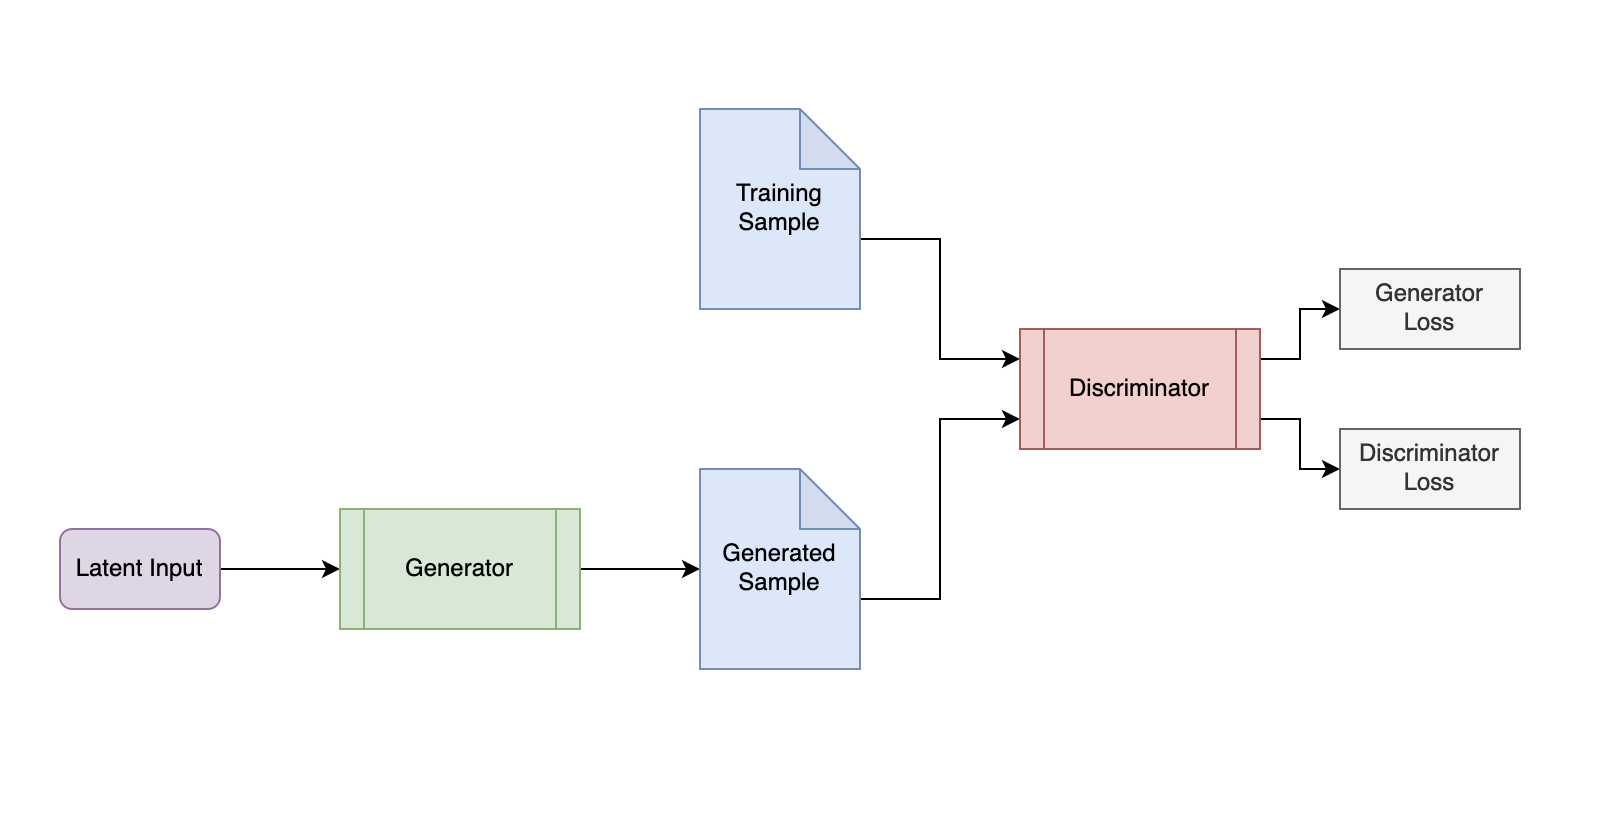
\includegraphics[width=\columnwidth]{images/gan_architecture.png}}
\caption{Architecture of Generative Adversarial Network}
\label{gan-architecture}
\end{center}
\vskip -0.2in
\end{figure}

I adopted a GAN architecture as shown in Figure \ref{gan-architecture}, comprising a generator and a discriminator with multiple layers. Leaky ReLU activation functions were used in the discriminator and the generator. The generator also had some batch normalization layers. Adam optimizer was used for both the generator and discriminator, with a single learning rate and momentum parameters. The model was trained using stochastic gradient descent for a fixed number of epochs.

\subsection{Implementation of VAE}
\begin{figure}[ht]
\vskip 0.2in
\begin{center}
\centerline{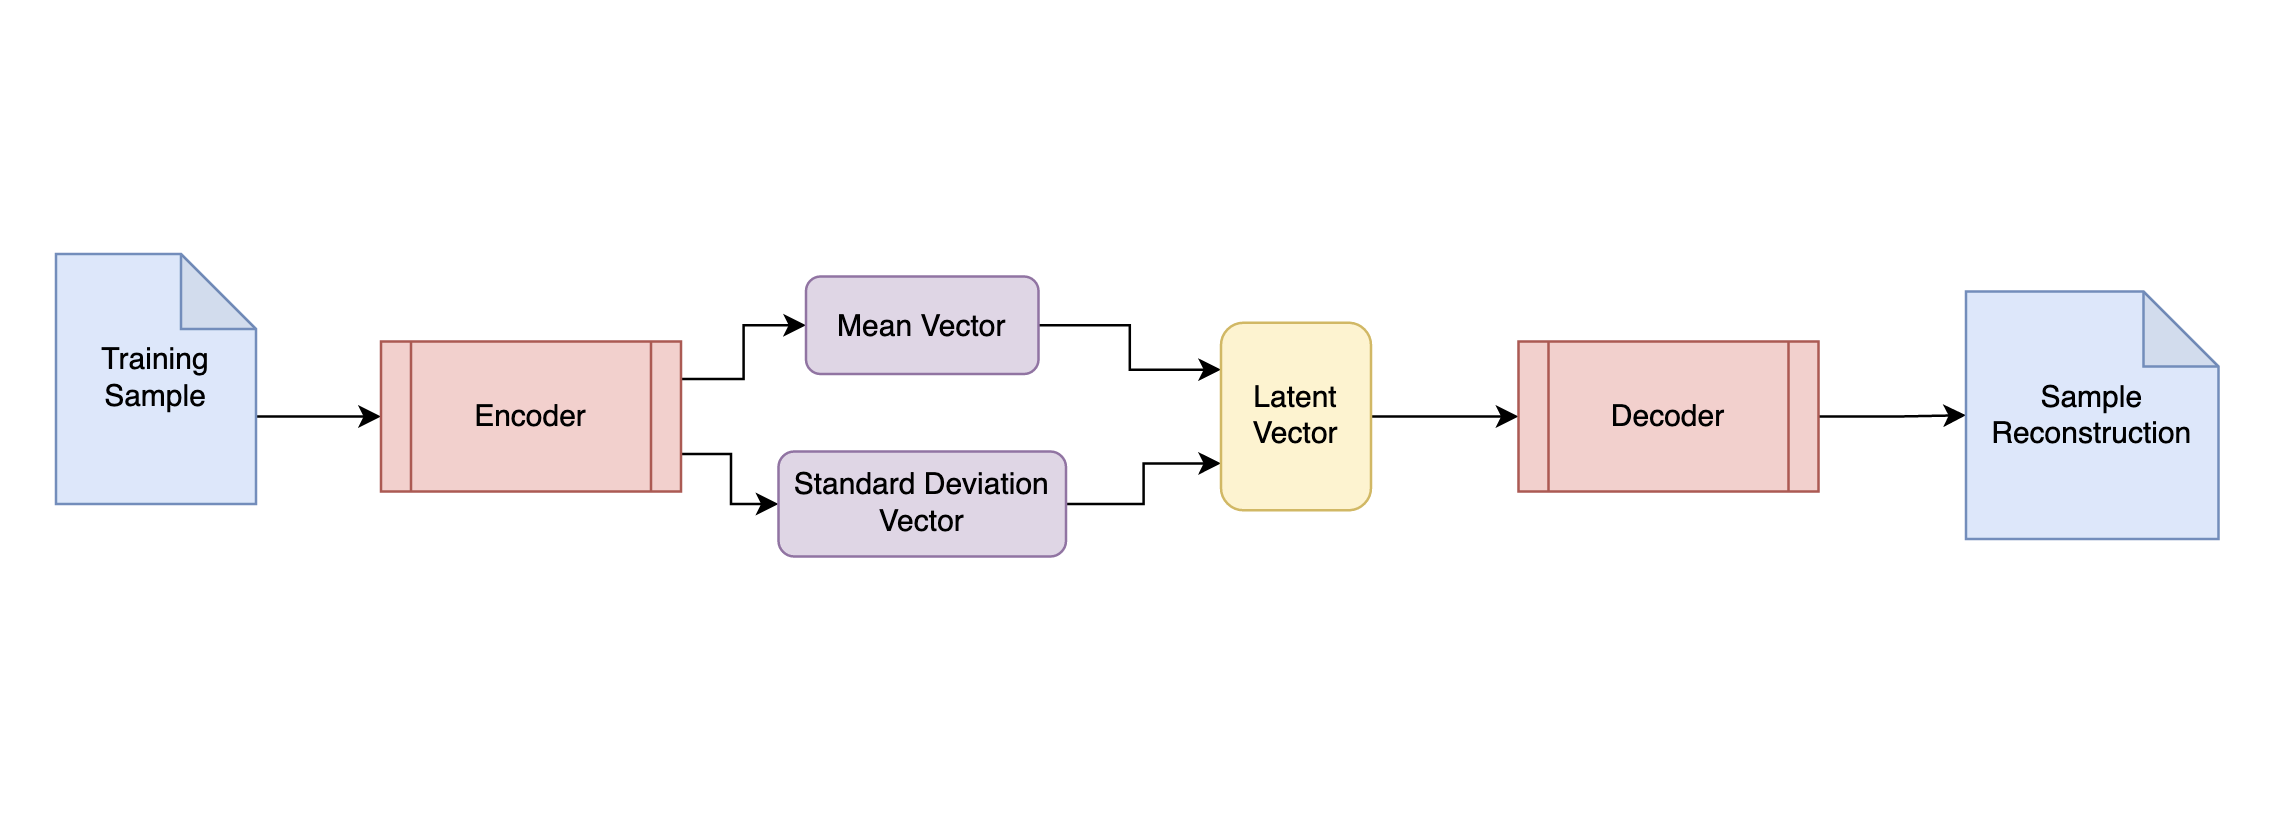
\includegraphics[width=\columnwidth]{images/vae_architecture.png}}
\caption{Architecture of Variational Autoencoder}
\label{vae-architecture}
\end{center}
\vskip -0.2in
\end{figure}
I adopted a VAE arechitecture as shown in Figure \ref{vae-architecture}, consisting of an encoder and a decoder with multiple layers. ReLU activation functions were used in both the encoder and decoder. The loss function was a combination of pixel-wise binary cross-entropy reconstruction loss and KL-divergence to encourage a structured latent space. The Adam optimizer was used for both the encoder and decoder, with a single learning rate and momentum parameters. The model was trained using stochastic gradient descent for a fixed number of epochs.

\subsection{Evaluation Metrics}
The performance of GANs and VAEs was evaluated using a combination of quantitative metrics (Reconstruction Loss in case of VAE) and qualitative assessments (latent space analysis and visual inspection).

\subsection{Hyperparameters}
Both models were trained for $100$ epochs with a Batch Size of $128$ and a Learning Rate of $0.001$. The total number of parameters for the GAN Generator, GAN Discriminator and VAE was $581264$, $566273$, and $849384$ respectively. Additionally, Binary Cross Entropy (BCE) Loss and ADAM optimizer ($\beta_1=0.5$, $\beta_2=0.9999$) was used for the GAN, and BCE + KLD Loss and ADAM optimizer ($\beta_1=0.5$, $\beta_2=0.9999$) was used for VAE.


\section{Results}
The results indicate that GANs are more suitable for generating high-quality, diverse, and visually appealing handwritten digits from the MNIST dataset, while VAEs demonstrate a stronger ability to capture the latent space and reconstruct input images. Figure \ref{gan-sample} and Figure \ref{vae-sample} display samples generated from GAN and VAE respectively.

\begin{figure}[ht]
\vskip 0.2in
\begin{center}
\centerline{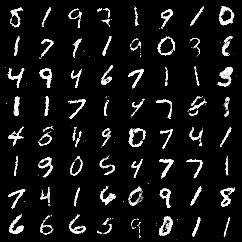
\includegraphics[width=\columnwidth]{images/gan_sample.png}}
\caption{64 Samples generated via GAN}
\label{gan-sample}
\end{center}
\vskip -0.2in
\end{figure}

\begin{figure}[ht]
\vskip 0.2in
\begin{center}
\centerline{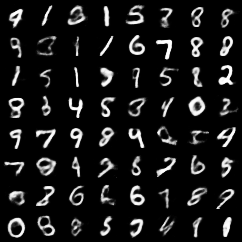
\includegraphics[width=\columnwidth]{images/vae_sample.png}}
\caption{64 Samples generated via VAE}
\label{vae-sample}
\end{center}
\vskip -0.2in
\end{figure}

\subsection{Quantitative Evaluation}
I reviewed some literature and found out that Inception Score and Fréchet Inception Distance are good metrics to evaluate the Quantitative Performance of GAN and VAE. However, I was not able to implement it in code successfully to be able to present the findings.

\subsection{GAN Performance and Findings}
The Generative Adversarial Network (GAN) was implemented and trained on the MNIST dataset to generate handwritten digits. After fine-tuning the model's hyperparameters, I observed that the GAN was capable of generating high-quality and diverse digit samples. The generated digits closely resembled the real data in terms of style, stroke thickness, and overall appearance.

\subsubsection{Qualitative Evaluation}
\begin{itemize}
    \item \textbf{Visual Inspection:} The visual inspection of generated images revealed high-quality samples with minimal noise and no apparent mode collapse.
\end{itemize}

\subsection{VAE Performance and Findings}
The Variational Autoencoder (VAE) was also implemented and trained on the MNIST dataset. The VAE demonstrated the ability to generate handwritten digits with varying levels of quality. The generated samples generally resembled real digits but were often blurrier compared to the GAN-generated images.

\begin{figure}[ht]
\vskip 0.2in
\begin{center}
\centerline{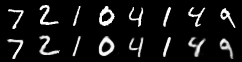
\includegraphics[width=\columnwidth]{images/vae_reconstruction.png}}
\caption{Test Sample (Above) and Reconstructed Sample (Below)}
\label{vae-reconstruction}
\end{center}
\vskip -0.2in
\end{figure}

\subsubsection{Quantitative Evaluation}
\begin{itemize}
    \item \textbf{Reconstruction Loss:} The VAE achieved a reconstruction loss of $95.832$, indicating its capability to accurately reconstruct input images as shown in Figure \ref{vae-reconstruction}.
\end{itemize}

\subsubsection{Qualitative Evaluation}
\begin{itemize}
    \item \textbf{Visual Inspection:} The visual inspection of generated images showed moderately realistic digits but with more noticeable artifacts and blurriness compared to the GAN-generated images.
\end{itemize}

\subsection{Interpolation Experiments}

I attempted to investigate the smoothness and continuity of the latent spaces learned by both the GAN and VAE models. I performed linear interpolations between pairs of randomly selected points in the latent space and decoded these interpolated points into images. Unfortunately, my interpolation experiments did not yield the desired outcomes for either model.

\begin{figure}[ht]
\vskip 0.2in
\begin{center}
\centerline{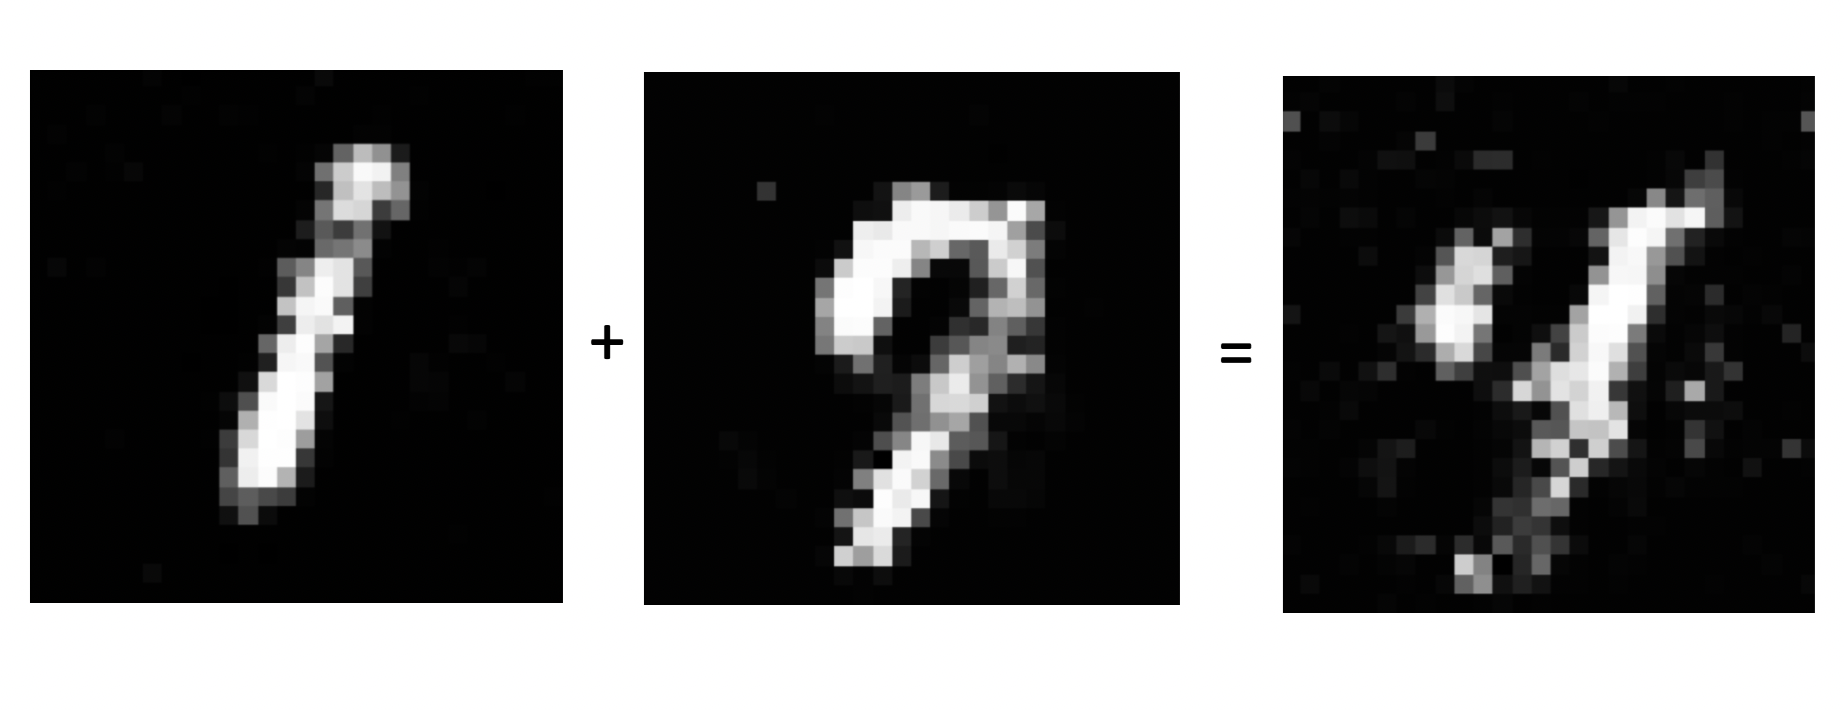
\includegraphics[width=\columnwidth]{images/gan_interpolation.png}}
\caption{Two points in latent space and decoded image of the resulting interpolated point for GAN }
\label{gan-interpolation}
\end{center}
\vskip -0.2in
\end{figure}

\begin{figure}[ht]
\vskip 0.2in
\begin{center}
\centerline{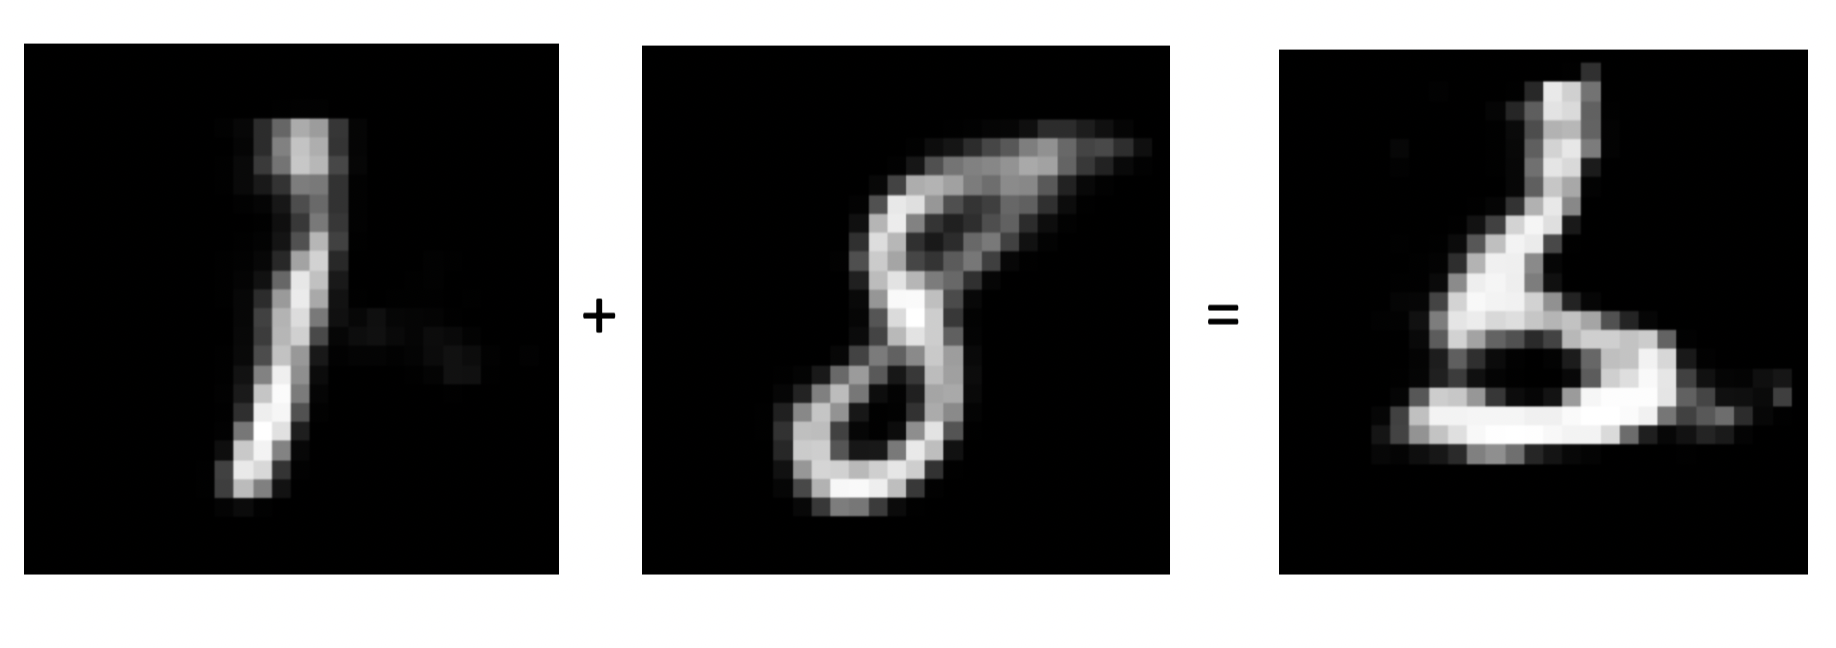
\includegraphics[width=\columnwidth]{images/vae_interpolation.png}}
\caption{Two points in latent space and decoded image of the resulting interpolated point for VAE }
\label{vae-interpolation}
\end{center}
\vskip -0.2in
\end{figure}

For the GAN, as shown in Figure \ref{gan-interpolation}, the generated images corresponding to interpolated points appeared to be unrealistic, containing noise. This result can be attributed to the fact that GANs typically focus on generating high-quality samples rather than ensuring a smooth latent space. As a result, the GAN's latent space might not be well-suited for interpolation tasks. Similarly, as shown in Figure \ref{vae-interpolation}, the VAE interpolation experiments also failed to produce satisfactory results. 

Despite the unsuccessful interpolation experiments, these findings provide valuable insights into the limitations of both GANs and VAEs in terms of their latent space properties and encourage further exploration of alternative generative models or techniques to improve the interpolation performance.

\subsection{Comparative Analysis of GAN and VAE}
Based on the evaluation metrics and visual inspection, I observed several key differences between the performance of GANs and VAEs:
\begin{itemize}
    \item \textbf{Image Quality:} GANs generated sharper and more realistic images compared to VAEs, which tended to produce blurrier samples.
    \item \textbf{Diversity:} Both models were capable of generating diverse samples.
    \item \textbf{Reconstruction Ability:} The VAE demonstrated a better ability to reconstruct input images, as shown by the lower reconstruction loss, while the GAN did not have an inherent mechanism for reconstruction.
\end{itemize}


\section{Difficulties and Challenges}
During the course of this project, various challenges and difficulties were encountered while implementing the Generative Adversarial Networks (GANs) and Variational Autoencoders (VAEs).

These difficulties and challenges gave me valuable insights into the practical aspects of implementing GANs and VAEs and highlighted potential areas for future research to improve the performance of the models.


\begin{figure}[ht]
\vskip 0.2in
\begin{center}
\centerline{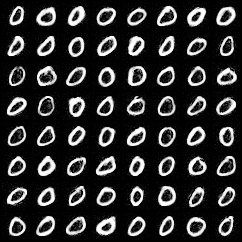
\includegraphics[width=\columnwidth]{images/gan_mode_collapse.png}}
\caption{GAN generating only $0$s after Mode Collapse}
\label{gan-mode-collapse}
\end{center}
\vskip -0.2in
\end{figure}

\begin{figure}[ht]
\vskip 0.2in
\begin{center}
\centerline{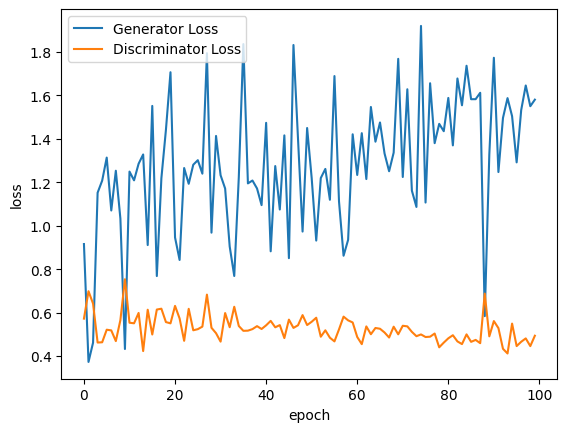
\includegraphics[width=\columnwidth]{images/gan_loss.png}}
\caption{GAN loss oscillating without convergence}
\label{gan-loss}
\end{center}
\vskip -0.2in
\end{figure}

\subsection{Difficulties in Generative Adversarial Networks}
\begin{itemize}
    \item \textbf{Mode Collapse:} One common issue I encountered with GANs was mode collapse as shown in Figure \ref{gan-mode-collapse}, where the generator produced a limited variety of samples, leading to a lack of diversity in the generated images. This issue required careful tuning of hyperparameters.
    \item \textbf{Training Stability:} GAN training was unstable, with the generator and discriminator oscillating between different states without convergence as shown in Figure \ref{gan-loss}. Ensuring the balance between the generator and discriminator during training required monitoring loss functions and adjusting learning rates.
    \item \textbf{Hyperparameter Tuning:} Finding the optimal set of hyperparameters for GANs was challenging and time-consuming. It required extensive experimentation and testing to achieve satisfactory performance.
\end{itemize}

\subsection{Difficulties in Variational Autoencoders}
\begin{itemize}
    \item \textbf{Blurry Images:} A recurring issue with VAE-generated images was their tendency to be blurrier compared to GAN-generated images. Exploring alternative loss functions or refining the architecture could potentially help improve image quality.
    \item \textbf{Model Divergence:} Initially I started with only pixel-wise BCE Loss but the results were very poor. I added KL-Divergence term to Loss to fix this issue.
    \item \textbf{Model Complexity:} I found the implementation of VAE to be trickier than the implementation of the GAN. This could be attributed to the fact that the VAE includes some probabilistic modelling as well.
\end{itemize}

\subsection{Difficulties in Comparative Study}
Ensuring a fair comparison between GANs and VAEs required maintaining consistency in experimental setups, such as dataset preparation, training procedures, and evaluation methodologies. This consistency was crucial in drawing meaningful conclusions from the comparative analysis.

\section{Future Work}
Future work in this project could focus on improving the performance of both GAN and VAE by exploring various data augmentation techniques. Data augmentation, which involves creating new training samples by applying transformations to the original dataset, has been shown to improve the generalization capabilities of deep learning models. By augmenting the MNIST dataset with rotated, scaled, and translated versions of the original images, it might be possible to encourage the models to learn more about the latent space. Various model ensemble methods could be explored in order to achieve better results by combining the strengths of the models.

\section{Conclusion}
This paper presented a  comparison of Generative Adversarial Networks (GANs) and Variational Autoencoders (VAEs) for generating handwritten digits from the MNIST dataset. The project involved the implementation and evaluation of both models, an analysis of the difficulties and challenges faced.

The results showed that GANs excel at producing high-quality, and diverse images, while VAEs demonstrated better reconstruction capabilities. The comparative study highlighted the unique strengths and weaknesses of each model, suggesting that they may be more suitable for specific applications depending on the desired outcomes.

Difficulties and challenges encountered during the research provided valuable insights into the practical aspects of implementing GANs and VAEs, such as dealing with mode collapse, training instability, and hyperparameter tuning.

In conclusion, this paper contributed to a deeper understanding of GANs and VAEs in the context of generating handwritten digits from the MNIST dataset. The comparative study and insights gained can inform future research efforts.

\bibliography{main.bib}
\bibliographystyle{icml2021}


\end{document}


% This document was modified from the file originally made available by
% Pat Langley and Andrea Danyluk for ICML-2K. This version was created
% by Iain Murray in 2018, and modified by Alexandre Bouchard in
% 2019 and 2021. Previous contributors include Dan Roy, Lise Getoor and Tobias
% Scheffer, which was slightly modified from the 2010 version by
% Thorsten Joachims & Johannes Fuernkranz, slightly modified from the
% 2009 version by Kiri Wagstaff and Sam Roweis's 2008 version, which is
% slightly modified from Prasad Tadepalli's 2007 version which is a
% lightly changed version of the previous year's version by Andrew
% Moore, which was in turn edited from those of Kristian Kersting and
% Codrina Lauth. Alex Smola contributed to the algorithmic style files.
